% Resumo editorado Congresso SBG 2026

\documentclass[twocolumn, A4]{article}

% Pacotes

% fonte
\usepackage[utf8]{inputenc}
\usepackage[TU]{fontenc}
%figuras
\usepackage{graphicx}
% links, metadados
\usepackage{hyperref}
% formatação
\usepackage{microtype}
% língua
\usepackage[brazil]{babel}
% referências
\usepackage[round, authoryear, sort]{natbib}
\bibliographystyle{unsrtnat}

% Links e metadados
\hypersetup{
	colorlinks,
	allcolors=blue,
	breaklinks=true,
	pdftitle={Reprodutibilidade de estudos sobre suscetibilidade à movimentos 
	de massa no Brasil: análise bibliométrica},
	pdfauthor={Samira Lisboa Santos, Carlos Henrique Grohmann}
}

\begin{document}

\title{Reprodutibilidade de estudos sobre suscetibilidade à movimentos de massa no Brasil: 
análise bibliométrica}
\author{
	Samira  Lisboa Santos\textsuperscript{1,3},
	Carlos Henrique Grohmann\textsuperscript{2,3}
 	\\[0.2cm]
	{\small \textsuperscript{1}Aluno de graduação no Instituto de Astronomia, Geofísica e Ciências Atmosféricas; email: saalisboas@usp.br} \\
	{\small \textsuperscript{2}Professor Titular do Instituto de Astronomia, Geofísica e Ciências Atmosféricas;} \\
	{\small \textsuperscript{3}Spatial Analysis And Modelling Lab (SPAMLab), Universidade de São Paulo, Brasil.}
}
\date{Setembro, 2026}

\maketitle
\newpage

\section{Resumo}
A disponibilidade é um dos principais meios da ciência aberta. Esta revisão bibliométrica almeja realizar um panorama da reprodutibilidade com a visibilidade de dados e códigos, para um grupo de artigos sobre susceptibilidade a escorregamentos de massa no Brasil. Após seleções prévias, analisa-se o ano de publicação, revista e número de citações. Além disso, a correspondência tanto na topografia quanto na demografia também é discutida.

\section{Introdução}
Movimentos de massa são processos geomorfológicos, influenciados por fatores geológicos, 
topográficos e climáticos da região \citep{Varnes1978}. A ocupação urbana desordenada 
em locais predispostos a tais ocorrências acarreta em acidentes e desastres; dessa forma,
a adoção de medidas preventivas pode agir na contenção de danos \citep{ConhecerPrevenir}. 

A análise de suscetibilidade a movimentos de massa é composta por dados de fatores 
ambientais ou desencadeantes, de elementos em risco e do inventário de escorregamentos 
\citep{VanWesten}, sendo este o principal, pois sua qualidade afeta a precisão 
dos resultados \citep{Steger20162729}. A utilização e reaproveitamento de inventários de 
qualidade permite, portanto, a comparação imparcial entre métodos de pesquisa 
\citep{Coelho2024}. 

O compartilhamento de dados pode contribuir na identificação de possíveis erros na 
análise ou de falsas conclusões \citep{Munafo2017}. Porém, facilitar a replicação de 
estudos é raro na literatura científica: a chamada ``crise de reprodutibilidade'' 
\citep{Baker2016}. 

Uma minoria de artigos busca o livre acesso dos dados, muitas vezes 
prometidos a partir de ``pedidos razoáveis'' e não obtidos na prática \citep{Tedersoo2021}. 
A solicitação de artigos não compartilhados diretamente é impedida por diversos fatores,
desde impossibilidade de contato ou obtenção dos dados a problemas pessoais ou profissionais,
o que torna pedir dados uma grande barreira \citep{Hussey}.

Assim, a proposta do projeto é avaliar a disponibilidade de dados em artigos de 
suscetibilidade à escorregamentos no território brasileiro. 

\section{Metodologia}
Todos os artigos estão no site Scopus, a partir de três pesquisas por palavras-chave. Cada resumo foi lido, selecionado e, caso fosse compatível com as áreas do lugar e do conhecimento de interesse, as informações extraídas para um arquivo .csv como banco de dados. Após conclusão, tal processo estará disponível no github.

Depois da análise completa dos dez estudos mais citados, um código python foi desenvolvido para procurar por termos frequentes e relacionar às informações do artigo. 

   \begin{figure}
        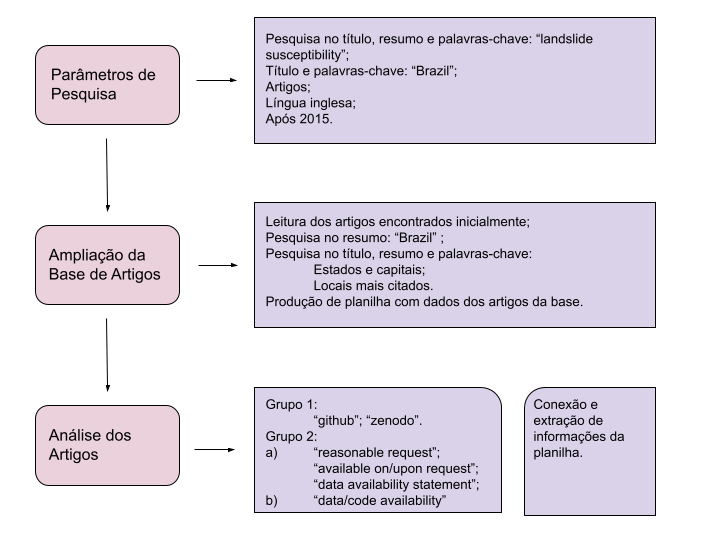
\includegraphics[width=\linewidth]{fluxograma.png}
        \caption{Fluxograma da filtragem, construção da base de dados e 
	análise dos artigos.}
        \label{fig:fluxo}
    \end{figure} 

Conforme análise de \citet{Dias2021}, a maior parte dos artigos brasileiros são escritos
em língua inglesa; isso foi confirmado em filtragens prévias de plataforma e, para
análise, optou-se por selecionar artigos em inglês. A ambrangência de dez anos, 
além de incluir a maior parte dos artigos disponíveis, coincide com o início da 
preocupação com o debate acerca de reprodutibilidade na ciência \citet{Baker2016}.

A busca por disponibilidade foi analisada caso a caso. Buscou-se, com isso, evitar possíveis 
coincidências de termos buscados sem relação com o tema. A pesquisa por termos
chave, escolhidos a partir de leitura e percepção de padrões na bibliografia,
foi feita em etapas para identificação de todos os artigos que mencionam 
disponibilidade, de qualquer forma. Optou-se pela busca primária do nome das plataformas 
online de dados e códigos por serem a forma mais comum de compartilhamento livre, 
conforme \citet{Tedersoo2021}. Aqueles que negam possibilidade de compartilhamento 
ou compartilham apenas materiais/softwares livres  utilizados, sem mencionar os próprios códigos e dados,
foram identificados para análise como não disponibilizadores de dados. 

Os critérios de disponibilidade utilizados foram:
\begin{itemize}
    \item não aberto; 
    \item disponível mediante pedido;
    \item aberto parcialmente; 
    \item totalmente disponível. 
\end{itemize}

A diferença entre as classes 3 e 4 se dá pelo real acesso ao repositório. Portanto, análises das informações secundárias foram realizadas paralelamente por leitura: levantamento de informações das revistas e métodos de pesquisa utilizados.

\section{Resultados}
Em cada uma das pesquisas, os artigos foram analisados em planilhas .csv de controle; aqueles com compatibilidade ao tema tiveram seus arquivos .pdf baixados. Para análise estatística de informações (ano, revista e número de citações) e
organização de referências utilizou-se a ferramenta de exportação da plataforma Scopus.

\subsection{Disponibilidade}
O código inicial de identificação em menção à disponibilidade retornou artigos que passaram à fase de leitura para conferência precisa. Esse retorno consistiu em três níveis, sendo buscados nos arquivos .pdf os termos:

\begin{itemize}
    \item `github', `zenodo'
    \item `data availability statement', `reasonable request', `available on request', `available upon request'
    \item `data availability', `code availability'
\end{itemize}
\begin{figure}
    \centering
    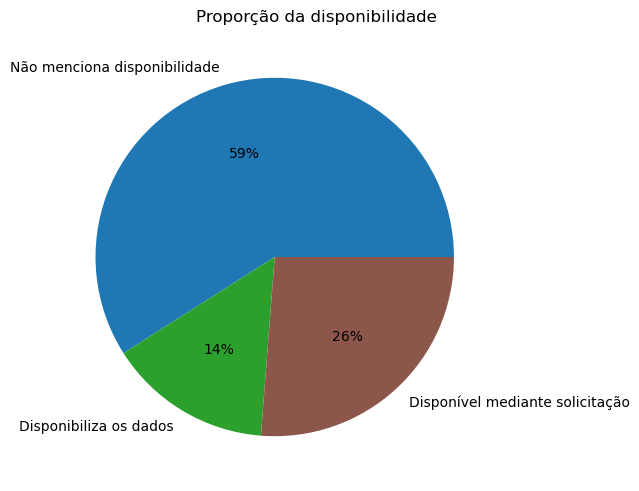
\includegraphics[width=\linewidth]{../figures/br-availability.png}
    \caption{A minoria dos artigos não menciona disponibilidade, e mesmo assim grande parte requer pedidos}
    \label{fig:dispon}
\end{figure}

\subsection{Informações correlatas}
A distribuição ao longo dos anos de debate acerca de disponibilidade
revelou que  mencionar o acesso aos dados foi implementado nos últimos 5 anos, tendo grande 
tendência em 2025, não prevista por anos anteriores (Figura \ref{fig:year}). Dos 61 artigos no banco de dados, apenas 25 têm código ou os dados disponíveis. Destes, todos são após 2020.

\begin{figure}
    \centering
    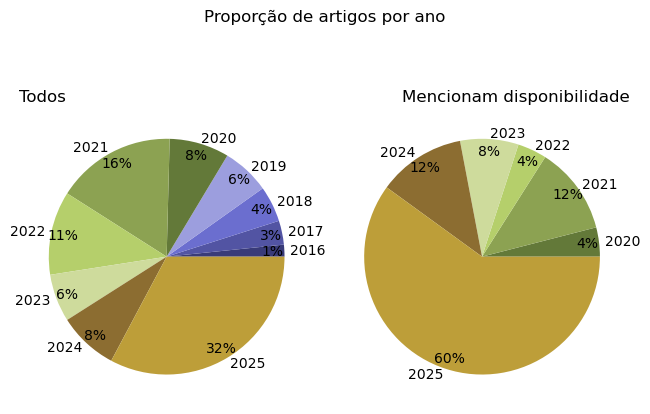
\includegraphics[width=\linewidth]{../figures/br-year.png}
    \caption{Mais da metade dos artigos que disponibilizam seus dados de alguma forma 
	são de 2025, sendo um terço da amostra de artigos desse ano}
    \label{fig:year}
\end{figure}

As revistas com mais publicações no assunto possuem artigos com disponibilidade, mesmo que por pedidos. Conforme já indicado por \citet{Munafo2017}, a política de ciência aberta da revista influencia significativamente na reprodutibilidade real dos artigos.
(Figura \ref{fig:journal}). \\

\begin{figure}
    \centering
    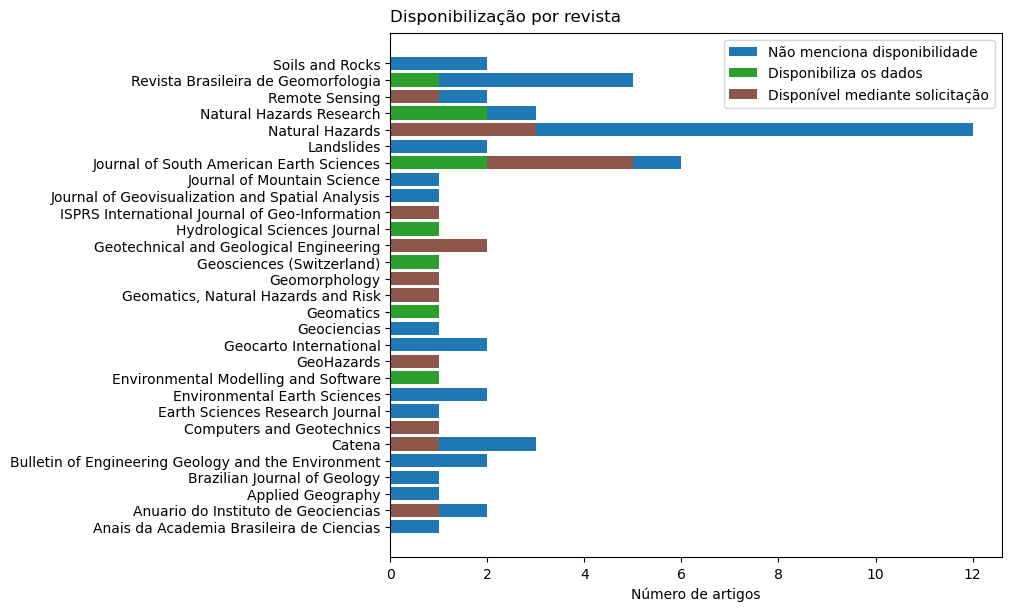
\includegraphics[width=\linewidth]{../figures/br-journal.png}
    \caption{Disponibilidade por revista}
    \label{fig:journal}
\end{figure}

A maioria dos artigos que mencionam a disponibilização de seus dados tem baixas citações,  
acompanhando a tendência geral. (Figura \ref{fig:cited}). Porém, a proporção de artigos com disponibilidade é maior entre os 5 mais citados em comparação ao restante de artigos.  Logo, não se observa relação estrita entre aumento de 
citações e compartilhamento de dados. Essa esperança também é discutida em \citet{Tedersoo2021}.

\begin{figure}
    \centering
    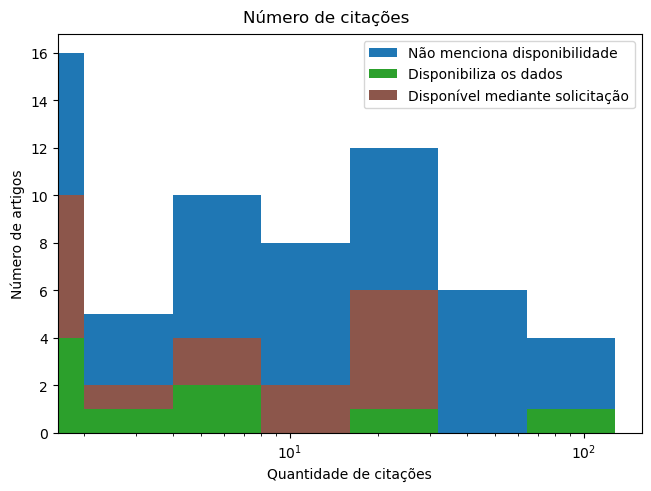
\includegraphics[width=\linewidth]{../figures/br-citations.png}
    \caption{Histograma de citações e disponibilidade}
    \label{fig:cited}
\end{figure}

 A análise de suscetibilidade é feita nos estudos principalmente por métodos estatísticos; ou seja, a indisponibilidade pode ser um enorme problema na qualidade da ciência reproduzível.
No Brasil, a densidade populacional histórica no sudeste pode afetar o interesse prioritário em estudos na Serra do Mar, pois tal tendência não é seguida por toda a Grande Escarpa. A completa disponibilidade foi concentrada em cidades densamente povoadas. 


\section{Conclusões}
A impressão de que a maioria dos artigos sobre suscetibilidade à movimento de massa no Brasil não disponibiliza seus dados ou seus códigos se confirmou. Menos da metade menciona disponibilidade, todos nos últimos cinco anos, majoritariamente em 2025. 
Não foram observadas diferenças no número de citações, mas a maioria dos artigos classificados como abertos foram publicados em revistas que incentivam práticas de ciência aberta.

O compartilhamento de dados é um tema central em discussões sobre reprodutibilidade e ciência aberta. Procura-se incentivar tais práticas institucional ou cientificamente e indica-se sucesso em políticas internas das revistas. Já a esperança de aumento no número de citações não se confirmou. 
A regionalização dos estudos também se demonstrou central, estando os artigos associados a locais com densidade populacional e universidades próximas.

\nocite{*}
\bibliography{intro-refs, br.bib}

\end{document}
